
\begin{figure}[H]
\centering
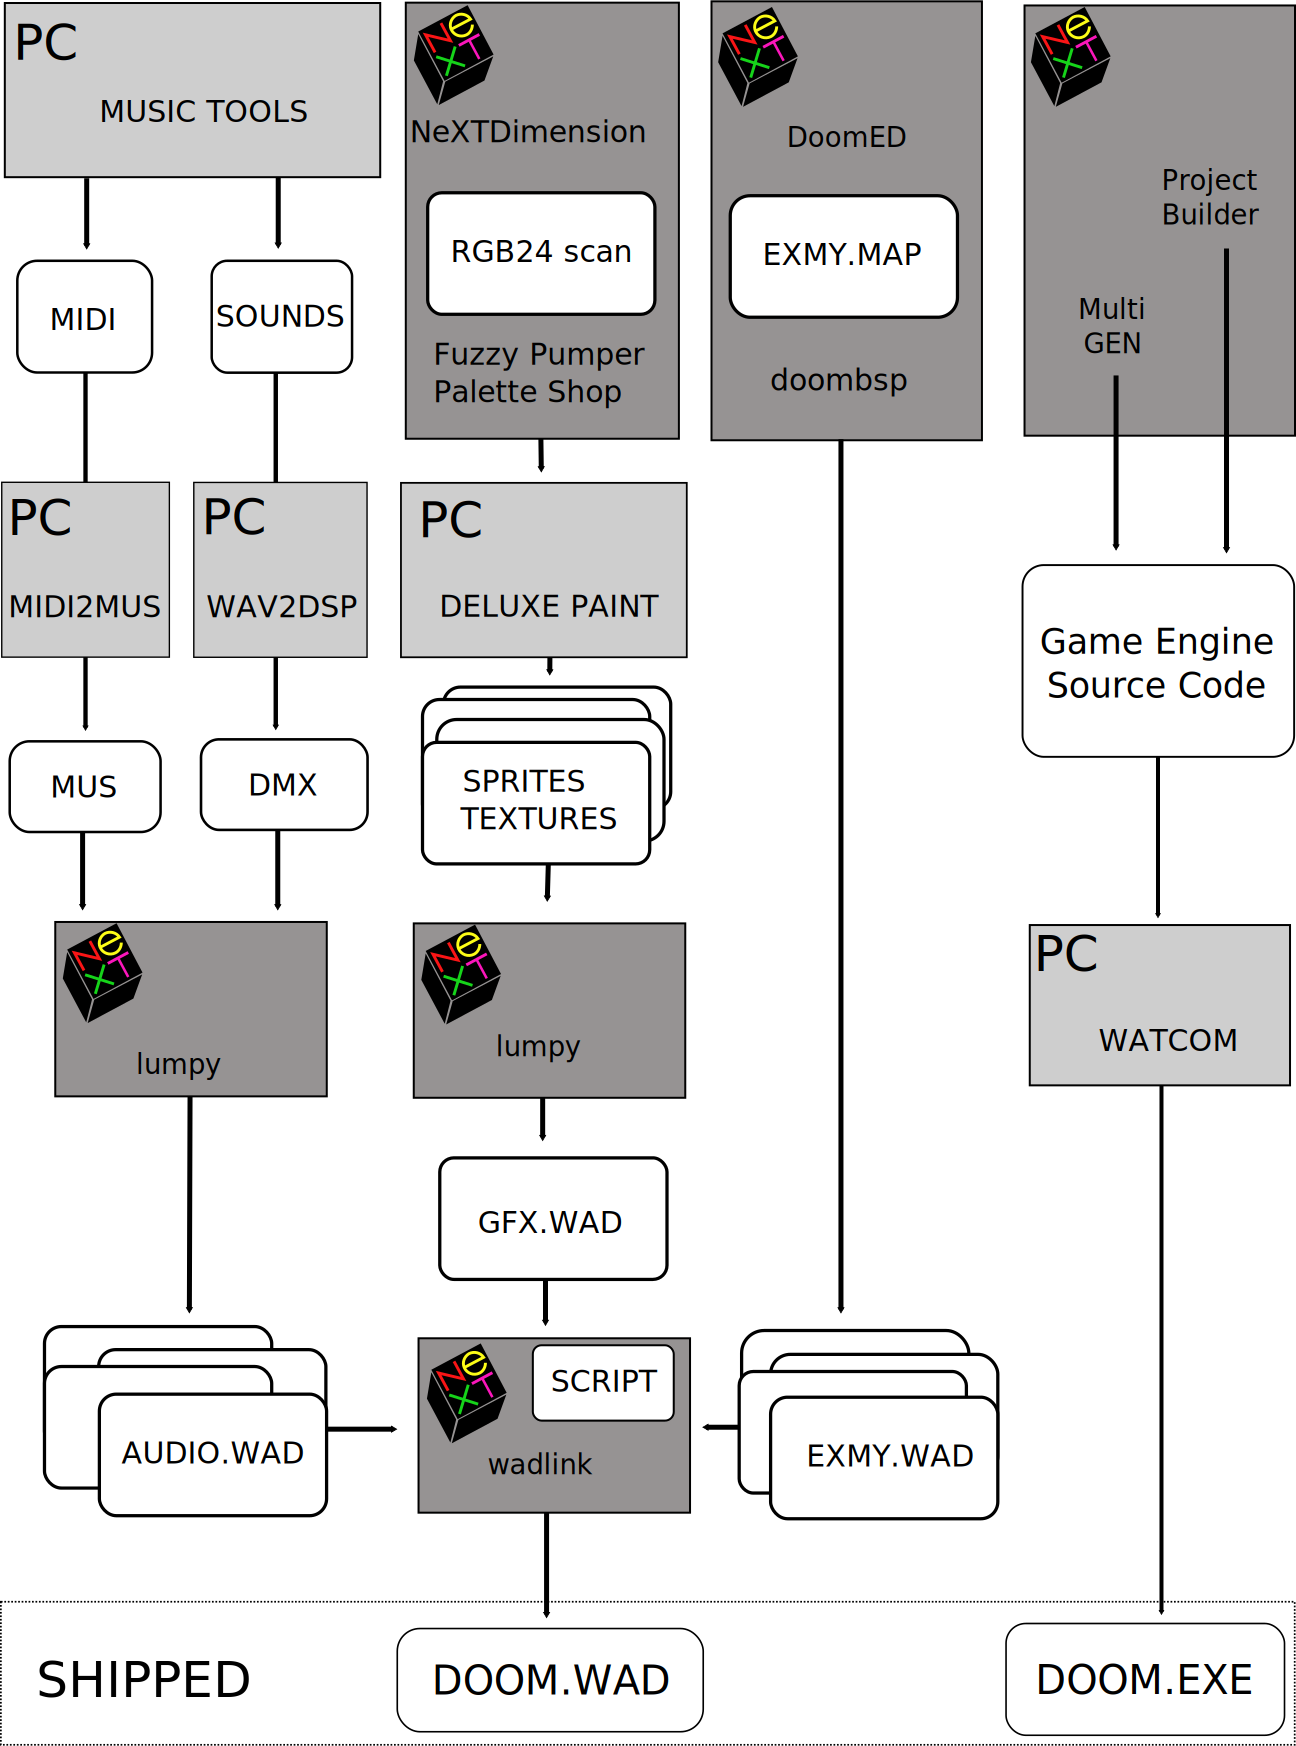
\includegraphics[width=\textwidth]{drawings/doom_pipeline.pdf}
\caption{Doom assets pipeline.}
\end{figure}
\par

\section{doombsp}
\cfullimage{doombsp_compiling.png}{}
\par
\cfullimage{doombsp_run.png}{}
\par


\section{DoomED}
\section{Fuzzy Pumper Palette Shop}
\section{Sprites}

Seven Doom characters were built as sculptures during Doom \& Doom II development. The first models - the Doomguy, baron of hell and cyberdemon -- were sculpted by Adrian Carmack. 

\scaledimage{0.4}{sprites/doomguy_sketch.png} 
\scaledimage{0.5}{sprites/doomguy_clay.png}\\
\par
\fullimage{sprites/doomguy_fpps.png}\\

\fullimage{sprites/adrian_hellknight.png}\\
\par
\fullimage{sprites/hellknight_fpps.png}\\
\par
\trivia{Mold Wooden Manikin}\\
\trivia{Most models survived. Some are still in John Romero possession while others are visible at XXX.}\\
\par
\trivia{Some complicated models such as the SpiderDemon where commissioned to Gregor Punchatz to build the rest of the models (the arch-vile, mancubus, revenant and spiderdemon). This was not Gregor's first gig since he had worked on major Hollywood movies such as Robocop before.}
\par
\fq{The spider creature was made out of parts I had literally just found at hardware and hobby stores, pieces of Tupperware and PVC pipes. The main body started out as a sculpture, then a plaster mold was pulled from that. Then we made the armature to fit that mold, and then foam latex was injected inside the mould and put into an oven.\\
\par
Mastermind's legs pretty much only just moved, and his arms moved, but his mouth didn’t move. As we went along, the other maquettes become full ball and socket armatures, so they had a full range of motion. In some ways, these stop-motion maquettes are easier to get right than they would be in CG. You don’t have to worry about how your skin is weighted on stop-motion model because it just sticks to the metal armature.}{Greg Punchatz\footnote{Interview by develop-online.net Feb 16, 2016}}\\
\par

\fq{At one stage id offered me points on the backend to take \$500 off the price of one of the characters and I turned that down. It’s a painful lesson. But to be part of something that has left a long-lasting impression on the world is kind of crazy – people find out that I worked on Doom and it’s like I played on the Beatles’ White Album.}{Greg Punchatz\footnote{Interview by develop-online.net Feb 16, 2016}}

\fullimage{sprites/spiderdemon_model.png}

Clay scupltures were photographed from eight different directions. The digitized version were then recolored automatically with Fuzzy Pumper Palette Shop. This process saved a lot of time for the artists since they only had to draw an unit once and sculpt it once.
\section{Props}
\fullimage{props/tom.png}\\
\fullimage{props/chainsaw.png}\\

\par
\trivia{To help convert code between NeXT and DOS, they wrote a tool named \cw{removecontrolm} and \cw{unfuck}}

\section{Sound effects}
bla
\section{Musics}
bla